% Created by tikzDevice version 0.12.3 on 2019-08-15 12:03:19
% !TEX encoding = UTF-8 Unicode
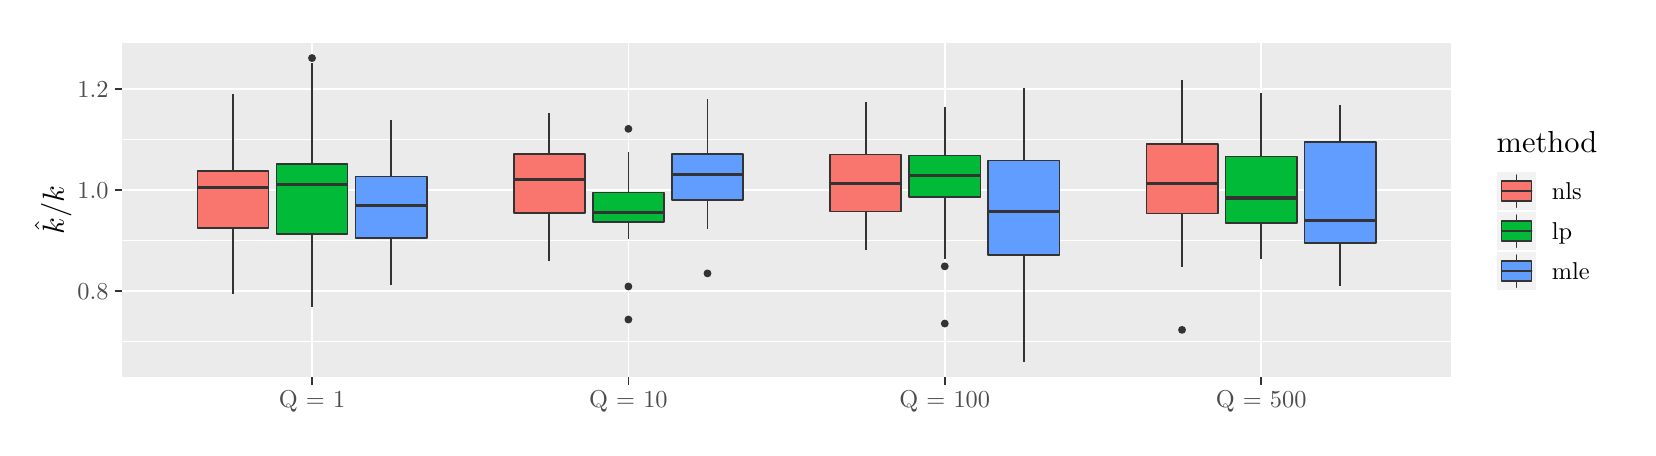
\begin{tikzpicture}[x=1pt,y=1pt]
\definecolor{fillColor}{RGB}{255,255,255}
\path[use as bounding box,fill=fillColor,fill opacity=0.00] (0,0) rectangle (578.16,144.54);
\begin{scope}
\path[clip] (  0.00,  0.00) rectangle (578.16,144.54);
\definecolor{drawColor}{RGB}{255,255,255}
\definecolor{fillColor}{RGB}{255,255,255}

\path[draw=drawColor,line width= 0.6pt,line join=round,line cap=round,fill=fillColor] (  0.00,  0.00) rectangle (578.16,144.54);
\end{scope}
\begin{scope}
\path[clip] ( 34.16, 18.22) rectangle (514.31,139.04);
\definecolor{fillColor}{gray}{0.92}

\path[fill=fillColor] ( 34.16, 18.22) rectangle (514.31,139.04);
\definecolor{drawColor}{RGB}{255,255,255}

\path[draw=drawColor,line width= 0.3pt,line join=round] ( 34.16, 31.17) --
	(514.31, 31.17);

\path[draw=drawColor,line width= 0.3pt,line join=round] ( 34.16, 67.65) --
	(514.31, 67.65);

\path[draw=drawColor,line width= 0.3pt,line join=round] ( 34.16,104.14) --
	(514.31,104.14);

\path[draw=drawColor,line width= 0.6pt,line join=round] ( 34.16, 49.41) --
	(514.31, 49.41);

\path[draw=drawColor,line width= 0.6pt,line join=round] ( 34.16, 85.89) --
	(514.31, 85.89);

\path[draw=drawColor,line width= 0.6pt,line join=round] ( 34.16,122.38) --
	(514.31,122.38);

\path[draw=drawColor,line width= 0.6pt,line join=round] (102.75, 18.22) --
	(102.75,139.04);

\path[draw=drawColor,line width= 0.6pt,line join=round] (217.07, 18.22) --
	(217.07,139.04);

\path[draw=drawColor,line width= 0.6pt,line join=round] (331.39, 18.22) --
	(331.39,139.04);

\path[draw=drawColor,line width= 0.6pt,line join=round] (445.71, 18.22) --
	(445.71,139.04);
\definecolor{drawColor}{gray}{0.20}

\path[draw=drawColor,line width= 0.6pt,line join=round] ( 74.17, 92.66) -- ( 74.17,120.51);

\path[draw=drawColor,line width= 0.6pt,line join=round] ( 74.17, 72.10) -- ( 74.17, 48.15);
\definecolor{fillColor}{RGB}{248,118,109}

\path[draw=drawColor,line width= 0.6pt,line join=round,line cap=round,fill=fillColor] ( 61.31, 92.66) --
	( 61.31, 72.10) --
	( 87.03, 72.10) --
	( 87.03, 92.66) --
	( 61.31, 92.66) --
	cycle;

\path[draw=drawColor,line width= 1.1pt,line join=round] ( 61.31, 86.68) -- ( 87.03, 86.68);
\definecolor{fillColor}{gray}{0.20}

\path[draw=drawColor,line width= 0.4pt,line join=round,line cap=round,fill=fillColor] (102.75,133.55) circle (  1.21);

\path[draw=drawColor,line width= 0.6pt,line join=round] (102.75, 95.23) -- (102.75,131.86);

\path[draw=drawColor,line width= 0.6pt,line join=round] (102.75, 69.87) -- (102.75, 43.51);
\definecolor{fillColor}{RGB}{0,186,56}

\path[draw=drawColor,line width= 0.6pt,line join=round,line cap=round,fill=fillColor] ( 89.89, 95.23) --
	( 89.89, 69.87) --
	(115.61, 69.87) --
	(115.61, 95.23) --
	( 89.89, 95.23) --
	cycle;

\path[draw=drawColor,line width= 1.1pt,line join=round] ( 89.89, 87.89) -- (115.61, 87.89);

\path[draw=drawColor,line width= 0.6pt,line join=round] (131.33, 90.72) -- (131.33,111.17);

\path[draw=drawColor,line width= 0.6pt,line join=round] (131.33, 68.60) -- (131.33, 51.44);
\definecolor{fillColor}{RGB}{97,156,255}

\path[draw=drawColor,line width= 0.6pt,line join=round,line cap=round,fill=fillColor] (118.47, 90.72) --
	(118.47, 68.60) --
	(144.19, 68.60) --
	(144.19, 90.72) --
	(118.47, 90.72) --
	cycle;

\path[draw=drawColor,line width= 1.1pt,line join=round] (118.47, 80.27) -- (144.19, 80.27);

\path[draw=drawColor,line width= 0.6pt,line join=round] (188.49, 98.83) -- (188.49,113.70);

\path[draw=drawColor,line width= 0.6pt,line join=round] (188.49, 77.54) -- (188.49, 60.16);
\definecolor{fillColor}{RGB}{248,118,109}

\path[draw=drawColor,line width= 0.6pt,line join=round,line cap=round,fill=fillColor] (175.63, 98.83) --
	(175.63, 77.54) --
	(201.35, 77.54) --
	(201.35, 98.83) --
	(175.63, 98.83) --
	cycle;

\path[draw=drawColor,line width= 1.1pt,line join=round] (175.63, 89.77) -- (201.35, 89.77);
\definecolor{fillColor}{gray}{0.20}

\path[draw=drawColor,line width= 0.4pt,line join=round,line cap=round,fill=fillColor] (217.07,107.98) circle (  1.21);

\path[draw=drawColor,line width= 0.4pt,line join=round,line cap=round,fill=fillColor] (217.07, 39.07) circle (  1.21);

\path[draw=drawColor,line width= 0.4pt,line join=round,line cap=round,fill=fillColor] (217.07, 51.01) circle (  1.21);

\path[draw=drawColor,line width= 0.6pt,line join=round] (217.07, 84.93) -- (217.07, 99.60);

\path[draw=drawColor,line width= 0.6pt,line join=round] (217.07, 74.28) -- (217.07, 68.03);
\definecolor{fillColor}{RGB}{0,186,56}

\path[draw=drawColor,line width= 0.6pt,line join=round,line cap=round,fill=fillColor] (204.21, 84.93) --
	(204.21, 74.28) --
	(229.93, 74.28) --
	(229.93, 84.93) --
	(204.21, 84.93) --
	cycle;

\path[draw=drawColor,line width= 1.1pt,line join=round] (204.21, 77.86) -- (229.93, 77.86);
\definecolor{fillColor}{gray}{0.20}

\path[draw=drawColor,line width= 0.4pt,line join=round,line cap=round,fill=fillColor] (245.65, 55.75) circle (  1.21);

\path[draw=drawColor,line width= 0.6pt,line join=round] (245.65, 98.94) -- (245.65,118.60);

\path[draw=drawColor,line width= 0.6pt,line join=round] (245.65, 82.25) -- (245.65, 71.71);
\definecolor{fillColor}{RGB}{97,156,255}

\path[draw=drawColor,line width= 0.6pt,line join=round,line cap=round,fill=fillColor] (232.79, 98.94) --
	(232.79, 82.25) --
	(258.51, 82.25) --
	(258.51, 98.94) --
	(232.79, 98.94) --
	cycle;

\path[draw=drawColor,line width= 1.1pt,line join=round] (232.79, 91.45) -- (258.51, 91.45);

\path[draw=drawColor,line width= 0.6pt,line join=round] (302.81, 98.75) -- (302.81,117.83);

\path[draw=drawColor,line width= 0.6pt,line join=round] (302.81, 78.16) -- (302.81, 64.14);
\definecolor{fillColor}{RGB}{248,118,109}

\path[draw=drawColor,line width= 0.6pt,line join=round,line cap=round,fill=fillColor] (289.95, 98.75) --
	(289.95, 78.16) --
	(315.67, 78.16) --
	(315.67, 98.75) --
	(289.95, 98.75) --
	cycle;

\path[draw=drawColor,line width= 1.1pt,line join=round] (289.95, 88.37) -- (315.67, 88.37);
\definecolor{fillColor}{gray}{0.20}

\path[draw=drawColor,line width= 0.4pt,line join=round,line cap=round,fill=fillColor] (331.39, 37.62) circle (  1.21);

\path[draw=drawColor,line width= 0.4pt,line join=round,line cap=round,fill=fillColor] (331.39, 58.29) circle (  1.21);

\path[draw=drawColor,line width= 0.6pt,line join=round] (331.39, 98.39) -- (331.39,115.80);

\path[draw=drawColor,line width= 0.6pt,line join=round] (331.39, 83.42) -- (331.39, 61.01);
\definecolor{fillColor}{RGB}{0,186,56}

\path[draw=drawColor,line width= 0.6pt,line join=round,line cap=round,fill=fillColor] (318.53, 98.39) --
	(318.53, 83.42) --
	(344.25, 83.42) --
	(344.25, 98.39) --
	(318.53, 98.39) --
	cycle;

\path[draw=drawColor,line width= 1.1pt,line join=round] (318.53, 91.23) -- (344.25, 91.23);

\path[draw=drawColor,line width= 0.6pt,line join=round] (359.97, 96.57) -- (359.97,122.90);

\path[draw=drawColor,line width= 0.6pt,line join=round] (359.97, 62.42) -- (359.97, 23.71);
\definecolor{fillColor}{RGB}{97,156,255}

\path[draw=drawColor,line width= 0.6pt,line join=round,line cap=round,fill=fillColor] (347.11, 96.57) --
	(347.11, 62.42) --
	(372.83, 62.42) --
	(372.83, 96.57) --
	(347.11, 96.57) --
	cycle;

\path[draw=drawColor,line width= 1.1pt,line join=round] (347.11, 78.16) -- (372.83, 78.16);
\definecolor{fillColor}{gray}{0.20}

\path[draw=drawColor,line width= 0.4pt,line join=round,line cap=round,fill=fillColor] (417.13, 35.34) circle (  1.21);

\path[draw=drawColor,line width= 0.6pt,line join=round] (417.13,102.41) -- (417.13,125.53);

\path[draw=drawColor,line width= 0.6pt,line join=round] (417.13, 77.35) -- (417.13, 58.19);
\definecolor{fillColor}{RGB}{248,118,109}

\path[draw=drawColor,line width= 0.6pt,line join=round,line cap=round,fill=fillColor] (404.27,102.41) --
	(404.27, 77.35) --
	(430.00, 77.35) --
	(430.00,102.41) --
	(404.27,102.41) --
	cycle;

\path[draw=drawColor,line width= 1.1pt,line join=round] (404.27, 88.38) -- (430.00, 88.38);

\path[draw=drawColor,line width= 0.6pt,line join=round] (445.71, 98.00) -- (445.71,120.77);

\path[draw=drawColor,line width= 0.6pt,line join=round] (445.71, 74.06) -- (445.71, 61.03);
\definecolor{fillColor}{RGB}{0,186,56}

\path[draw=drawColor,line width= 0.6pt,line join=round,line cap=round,fill=fillColor] (432.85, 98.00) --
	(432.85, 74.06) --
	(458.58, 74.06) --
	(458.58, 98.00) --
	(432.85, 98.00) --
	cycle;

\path[draw=drawColor,line width= 1.1pt,line join=round] (432.85, 82.99) -- (458.58, 82.99);

\path[draw=drawColor,line width= 0.6pt,line join=round] (474.29,103.11) -- (474.29,116.69);

\path[draw=drawColor,line width= 0.6pt,line join=round] (474.29, 66.69) -- (474.29, 51.36);
\definecolor{fillColor}{RGB}{97,156,255}

\path[draw=drawColor,line width= 0.6pt,line join=round,line cap=round,fill=fillColor] (461.43,103.11) --
	(461.43, 66.69) --
	(487.16, 66.69) --
	(487.16,103.11) --
	(461.43,103.11) --
	cycle;

\path[draw=drawColor,line width= 1.1pt,line join=round] (461.43, 74.78) -- (487.16, 74.78);
\end{scope}
\begin{scope}
\path[clip] (  0.00,  0.00) rectangle (578.16,144.54);
\definecolor{drawColor}{gray}{0.30}

\node[text=drawColor,anchor=base east,inner sep=0pt, outer sep=0pt, scale=  0.88] at ( 29.21, 46.38) {0.8};

\node[text=drawColor,anchor=base east,inner sep=0pt, outer sep=0pt, scale=  0.88] at ( 29.21, 82.86) {1.0};

\node[text=drawColor,anchor=base east,inner sep=0pt, outer sep=0pt, scale=  0.88] at ( 29.21,119.35) {1.2};
\end{scope}
\begin{scope}
\path[clip] (  0.00,  0.00) rectangle (578.16,144.54);
\definecolor{drawColor}{gray}{0.20}

\path[draw=drawColor,line width= 0.6pt,line join=round] ( 31.41, 49.41) --
	( 34.16, 49.41);

\path[draw=drawColor,line width= 0.6pt,line join=round] ( 31.41, 85.89) --
	( 34.16, 85.89);

\path[draw=drawColor,line width= 0.6pt,line join=round] ( 31.41,122.38) --
	( 34.16,122.38);
\end{scope}
\begin{scope}
\path[clip] (  0.00,  0.00) rectangle (578.16,144.54);
\definecolor{drawColor}{gray}{0.20}

\path[draw=drawColor,line width= 0.6pt,line join=round] (102.75, 15.47) --
	(102.75, 18.22);

\path[draw=drawColor,line width= 0.6pt,line join=round] (217.07, 15.47) --
	(217.07, 18.22);

\path[draw=drawColor,line width= 0.6pt,line join=round] (331.39, 15.47) --
	(331.39, 18.22);

\path[draw=drawColor,line width= 0.6pt,line join=round] (445.71, 15.47) --
	(445.71, 18.22);
\end{scope}
\begin{scope}
\path[clip] (  0.00,  0.00) rectangle (578.16,144.54);
\definecolor{drawColor}{gray}{0.30}

\node[text=drawColor,anchor=base,inner sep=0pt, outer sep=0pt, scale=  0.88] at (102.75,  7.21) {Q = 1};

\node[text=drawColor,anchor=base,inner sep=0pt, outer sep=0pt, scale=  0.88] at (217.07,  7.21) {Q = 10};

\node[text=drawColor,anchor=base,inner sep=0pt, outer sep=0pt, scale=  0.88] at (331.39,  7.21) {Q = 100};

\node[text=drawColor,anchor=base,inner sep=0pt, outer sep=0pt, scale=  0.88] at (445.71,  7.21) {Q = 500};
\end{scope}
\begin{scope}
\path[clip] (  0.00,  0.00) rectangle (578.16,144.54);
\definecolor{drawColor}{RGB}{0,0,0}

\node[text=drawColor,rotate= 90.00,anchor=base,inner sep=0pt, outer sep=0pt, scale=  1.10] at ( 13.08, 78.63) {$\hat{k}/k$};
\end{scope}
\begin{scope}
\path[clip] (  0.00,  0.00) rectangle (578.16,144.54);
\definecolor{fillColor}{RGB}{255,255,255}

\path[fill=fillColor] (525.31, 43.84) rectangle (572.66,113.42);
\end{scope}
\begin{scope}
\path[clip] (  0.00,  0.00) rectangle (578.16,144.54);
\definecolor{drawColor}{RGB}{0,0,0}

\node[text=drawColor,anchor=base west,inner sep=0pt, outer sep=0pt, scale=  1.10] at (530.81, 99.27) {method};
\end{scope}
\begin{scope}
\path[clip] (  0.00,  0.00) rectangle (578.16,144.54);
\definecolor{drawColor}{RGB}{255,255,255}
\definecolor{fillColor}{gray}{0.95}

\path[draw=drawColor,line width= 0.6pt,line join=round,line cap=round,fill=fillColor] (530.81, 78.25) rectangle (545.26, 92.70);
\end{scope}
\begin{scope}
\path[clip] (  0.00,  0.00) rectangle (578.16,144.54);
\definecolor{drawColor}{gray}{0.20}

\path[draw=drawColor,line width= 0.6pt,line join=round,line cap=round] (538.03, 79.70) --
	(538.03, 81.86);

\path[draw=drawColor,line width= 0.6pt,line join=round,line cap=round] (538.03, 89.09) --
	(538.03, 91.26);
\definecolor{fillColor}{RGB}{248,118,109}

\path[draw=drawColor,line width= 0.6pt,line join=round,line cap=round,fill=fillColor] (532.61, 81.86) rectangle (543.45, 89.09);

\path[draw=drawColor,line width= 0.6pt,line join=round,line cap=round] (532.61, 85.48) --
	(543.45, 85.48);
\end{scope}
\begin{scope}
\path[clip] (  0.00,  0.00) rectangle (578.16,144.54);
\definecolor{drawColor}{RGB}{255,255,255}
\definecolor{fillColor}{gray}{0.95}

\path[draw=drawColor,line width= 0.6pt,line join=round,line cap=round,fill=fillColor] (530.81, 63.80) rectangle (545.26, 78.25);
\end{scope}
\begin{scope}
\path[clip] (  0.00,  0.00) rectangle (578.16,144.54);
\definecolor{drawColor}{gray}{0.20}

\path[draw=drawColor,line width= 0.6pt,line join=round,line cap=round] (538.03, 65.24) --
	(538.03, 67.41);

\path[draw=drawColor,line width= 0.6pt,line join=round,line cap=round] (538.03, 74.64) --
	(538.03, 76.81);
\definecolor{fillColor}{RGB}{0,186,56}

\path[draw=drawColor,line width= 0.6pt,line join=round,line cap=round,fill=fillColor] (532.61, 67.41) rectangle (543.45, 74.64);

\path[draw=drawColor,line width= 0.6pt,line join=round,line cap=round] (532.61, 71.02) --
	(543.45, 71.02);
\end{scope}
\begin{scope}
\path[clip] (  0.00,  0.00) rectangle (578.16,144.54);
\definecolor{drawColor}{RGB}{255,255,255}
\definecolor{fillColor}{gray}{0.95}

\path[draw=drawColor,line width= 0.6pt,line join=round,line cap=round,fill=fillColor] (530.81, 49.34) rectangle (545.26, 63.80);
\end{scope}
\begin{scope}
\path[clip] (  0.00,  0.00) rectangle (578.16,144.54);
\definecolor{drawColor}{gray}{0.20}

\path[draw=drawColor,line width= 0.6pt,line join=round,line cap=round] (538.03, 50.79) --
	(538.03, 52.96);

\path[draw=drawColor,line width= 0.6pt,line join=round,line cap=round] (538.03, 60.18) --
	(538.03, 62.35);
\definecolor{fillColor}{RGB}{97,156,255}

\path[draw=drawColor,line width= 0.6pt,line join=round,line cap=round,fill=fillColor] (532.61, 52.96) rectangle (543.45, 60.18);

\path[draw=drawColor,line width= 0.6pt,line join=round,line cap=round] (532.61, 56.57) --
	(543.45, 56.57);
\end{scope}
\begin{scope}
\path[clip] (  0.00,  0.00) rectangle (578.16,144.54);
\definecolor{drawColor}{RGB}{0,0,0}

\node[text=drawColor,anchor=base west,inner sep=0pt, outer sep=0pt, scale=  0.88] at (550.76, 82.45) {nls};
\end{scope}
\begin{scope}
\path[clip] (  0.00,  0.00) rectangle (578.16,144.54);
\definecolor{drawColor}{RGB}{0,0,0}

\node[text=drawColor,anchor=base west,inner sep=0pt, outer sep=0pt, scale=  0.88] at (550.76, 67.99) {lp};
\end{scope}
\begin{scope}
\path[clip] (  0.00,  0.00) rectangle (578.16,144.54);
\definecolor{drawColor}{RGB}{0,0,0}

\node[text=drawColor,anchor=base west,inner sep=0pt, outer sep=0pt, scale=  0.88] at (550.76, 53.54) {mle};
\end{scope}
\end{tikzpicture}
